\documentclass{standalone}
\usepackage{tikz}
\usetikzlibrary{patterns, angles}

\begin{document}
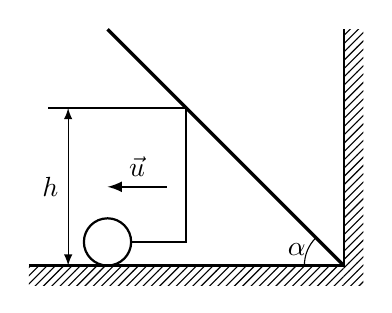
\begin{tikzpicture}
	\coordinate (A) at (1, 0);
    \coordinate (C) at (5, 0);
    \coordinate (D) at (5, 3);

    \coordinate (E) at (2, 3);
%    \coordinate (M) at (1.5, 1);
       
	\draw [draw=none, pattern=north east lines] (C) rectangle (1,-0.25);
	\draw [draw=none, pattern=north east lines] (5.25,-0.25) rectangle (D);	
	\draw [thick] (A) -- (C) -- (D);
	\draw [very thick] (C) -- (E);

%	\draw [very thick] (A) node [right=4pt, above] {$A$} -- (B) node [above] {$B$};
	\draw [thick] (1.25, 2) -- (3, 2) -- (3, 0.3) -- (2.3, 0.3);
	\draw [thick] (2, 0.3) circle (0.3);	
%	\draw [fill] (B) circle (0.05);
%	\draw [fill] (M) circle (0.05) node [right=2pt, above] {$M$};
	\pic [draw, -, angle eccentricity=1.5] {angle = E--C--A};
	\node [left=17pt, above] at (C) {$\alpha$};
	\draw [arrows={-latex}, thick] (2.75, 1) -- (2, 1) node [above, midway]  {$\vec{u}$};
	\draw [arrows={latex-latex}] (1.5, 0) -- (1.5, 2) node [midway, left]  {$h$};
\end{tikzpicture}
\end{document}